% ============================================================
% PART I OF THE SCIENTIFIC PROPOSAL (max. 5 pages)
% References do not count towards the page limit.
% ============================================================
% Header: Lepperød — FIND — Part B1

\section{Part I of the Scientific Proposal}

\begin{wrapfigure}{r}{0.50\textwidth}
    \vspace{-5mm}
    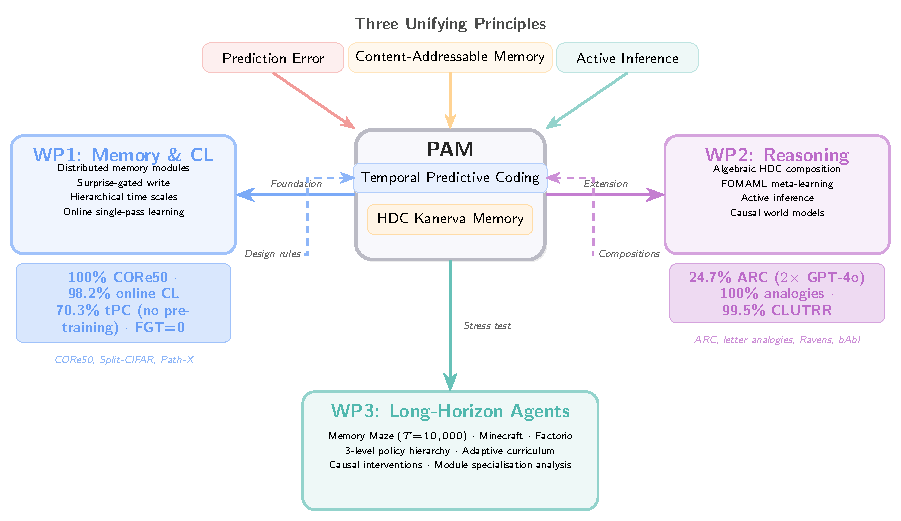
\includegraphics[trim=0mm 0mm 0mm 0mm, clip, width=0.50\textwidth]{figures/overview-find.pdf}
    \caption{\textbf{Conceptual overview of FIND.} PAM (centre) unifies temporal predictive coding, HDC-based content-addressable memory, and active inference under one prediction-error objective. Three work packages build outward: \textbf{WP1} establishes the memory and continual learning foundation; \textbf{WP2} extends with compositional reasoning and causal world models; \textbf{WP3} stress-tests in demanding long-horizon environments. Preliminary results (coloured boxes) validate each WP's core claims.}\label{fig:overview}
    \vspace{-4mm}
\end{wrapfigure}

We live in time. Memory bridges past and present, enabling agents to learn from experience and make informed decisions. Humans develop internal world models for planning and reasoning; replicating this in machines is the next step toward flexible AI~\cite{lecun2022path}.
Current AI struggles to generalise~\cite{razeghi2022impact}, lacking long-term memory~\cite{pasukonis2022evaluating}, causal understanding~\cite{richens2024robust}, and life-long learning without catastrophic forgetting~\cite{wang2024comprehensive}.

Consider an agent managing a Factorio production chain (Figure~\ref{fig:factorio}). It discovers copper wire requires copper plates (step~2,000) and circuits require wire plus iron (step~8,000), then encounters a blueprint requiring 50 circuits at step~15,000. It must recall the dependency chain across $>$10,000 timesteps, reason causally about bottlenecks, and adapt its layout. Current systems cannot do this: transformers trained from experience reach only $\sim$1{,}500-step memory and fail at long-horizon credit assignment~\cite{ni2023longterm}; SSMs compress dependencies into fixed-size state~\cite{gu2021s4}; MANNs lack causal models to identify bottlenecks~\cite{graves2016dnc}. The challenge is to achieve this \textit{learned from raw experience}, without a pretrained model or hand-engineered memory plumbing. \textbf{How can systems intelligently select what to retain, discard, and retrieve to learn across long temporal sequences?}

\begin{figure}[h!]
  \centering
  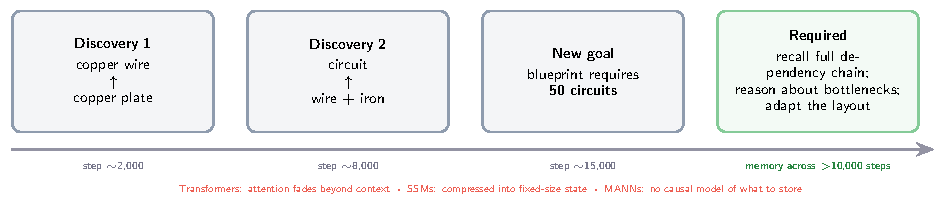
\includegraphics[width=\textwidth]{figures/factorio-storyboard.pdf}
  \caption{\textbf{The capability gap FIND addresses.} An agent discovers dependencies thousands of steps apart and must later recall and compose them under a new goal. This requires selective storage, content-addressable recall, and causal reasoning across $>$10,000 timesteps---beyond current architectures (bottom).}\label{fig:factorio}
\end{figure}

\subsection{Ground-breaking nature and impact}

FIND rests on a single bet: that predictive coding over distributed, content-addressable memory---the brain's mechanism for selective long-horizon recall---is the substrate flexible AI is missing. We develop \textbf{PAM} (\textbf{P}redictive \textbf{A}ctive \textbf{M}emory), a flat modular architecture built on one principle: \textbf{minimising prediction error over a shared memory}. That memory is a content-addressable distributed store~\cite{wu2018kanerva,kanerva2003sparse} whose contents are hyperdimensional vectors~\cite{kanerva2009hyperdimensional}, so recall and symbolic composition (binding, superposition) share one space. Every other mechanism is a way of touching that memory:
\begin{itemize}[noitemsep,topsep=2pt]
  \item \textbf{Encode:} temporal predictive coding denoises each observation into a clean latent before it is stored, so memory holds high-SNR content rather than raw input.
  \item \textbf{Retrieve:} content-addressable read by similarity, with HDC binding making retrieval compositional and symbolic.
  \item \textbf{Act:} active inference selects actions that bring incoming input into line with what memory predicts~\cite{friston2010free,rao2023active}, closing the perception--action loop on the same objective while gathering experience that updates memory.
\end{itemize}
\noindent Learned routing orchestrates which modules read and write when. The name is the thesis: a \textbf{P}redictive, \textbf{A}ctive \textbf{M}emory---predictive coding encodes, active inference acts, and content-addressable read retrieves.

\noindent\textbf{FIND's novelty} is this unification: it sits at the intersection of three established fields in a configuration no prior system has achieved simultaneously:
\begin{itemize}[noitemsep,topsep=2pt]
  \item \textbf{Temporal predictive coding}~\cite{millidge2024temporal} with \textbf{distributed external memory}---not just recurrent state: prior tPC models store context solely in hidden activations; FIND externalises memory into content-addressable HDC slots persistent across thousands of timesteps.
  \item \textbf{Memory-augmented networks}~\cite{graves2016dnc} with \textbf{biologically-grounded iterative inference}---not single-pass read/write: prior MANNs use a single forward pass to address memory; FIND uses iterative predictive-coding inference to resolve ambiguous queries against a content-addressable substrate (94\% exact recall at 32 stored pairs).
  \item \textbf{Hyperdimensional computing}~\cite{kanerva2009hyperdimensional} \textbf{embedded as the storage format of a gradient-trained system}---not as a standalone symbolic method: prior HDC systems operate outside neural training loops, and even NVSA~\cite{hersche2023nvsa}, which couples vector-symbolic reasoning to a trained perception network, is a single-task inference pipeline without persistent temporal memory, continual learning, or action; FIND makes HDC the storage substrate of a continual, temporal system, integrating binding directly into the memory update.
\end{itemize}

\noindent Table~\ref{tab:positioning} situates FIND against the state of the art: no existing system unites these capabilities in one end-to-end trainable architecture.

\begin{table}[h!]
\centering\footnotesize
\caption{\textbf{Positioning of PAM against existing approaches.} Only PAM combines external distributed memory, iterative inference, symbolic binding, and active inference in a single end-to-end trainable architecture.}\label{tab:positioning}
\vspace{2pt}
\begin{tabularx}{\textwidth}{@{}Xcccc@{}}
\toprule
\textbf{System} & \textbf{External Memory} & \textbf{Iterative Inference} & \textbf{Symbolic Binding} & \textbf{Active Inference} \\
\midrule
NTM / DNC~\cite{graves2014ntm,graves2016dnc} & \checkmark & --- & --- & --- \\
Kanerva Machine~\cite{wu2018kanerva} & \checkmark & --- & --- & --- \\
Temporal PC~\cite{millidge2024temporal} & --- & \checkmark & --- & --- \\
HDC systems~\cite{kanerva2009hyperdimensional} & --- & --- & \checkmark & --- \\
S4 / Mamba~\cite{gu2021s4} & --- (compressed state) & --- & --- & --- \\
Titans~\cite{behrouz2025titans} & \checkmark & --- & --- & --- \\
NVSA~\cite{hersche2023nvsa} & --- & --- & \checkmark & --- \\
Active PC~\cite{rao2023active} & --- & \checkmark & --- & \checkmark \\
\textbf{PAM (FIND)} & \textbf{\checkmark} & \textbf{\checkmark} & \textbf{\checkmark} & \textbf{\checkmark} \\
\bottomrule
\end{tabularx}
\end{table}

\subsection{State of the art, knowledge needs, and project objectives}

\subsubsection*{Temporal memory and predictive coding}

A key challenge in AI is creating memory systems comparable to the brain. RAG~\cite{lewis2020retrieval,yuan2024rag} and agentic systems like MemGPT~\cite{packer2024memgpt} manage context through external plumbing, but these sidestep bottom-up lifelong learning and struggle with out-of-distribution scenarios~\cite{razeghi2022impact}.

The core challenge is separating memory storage from computation~\cite{gemici2017generative,gallistel2011memory}. MANNs---NTMs~\cite{graves2014ntm}, DNCs~\cite{graves2016dnc}, Kanerva Machines~\cite{wu2018kanerva}---address this partially. HDC extends sparse distributed memories with symbolic binding~\cite{kanerva2009hyperdimensional,ma2022hyperbox}. Long-context transformers (Infini-Attention~\cite{munkhdalai2024infini}) extend windows but do not solve selective storage. Modern SSMs---Mamba-2~\cite{dao2024mamba2}, xLSTM~\cite{beck2024xlstm}---achieve efficient sequence processing but compress into fixed-size state.

Predictive coding (PC) minimizes prediction errors between expectations and inputs~\cite{millidge2022theoretical,friston2010free}. Extensions to active~\cite{rao2023active} and temporal PC~\cite{millidge2024temporal} enable biologically plausible cognitive maps. Test-time training (TTT)~\cite{sun2024ttt} shares PAM's iterative adaptation principle but modifies the full model rather than memory slots. Titans~\cite{behrouz2025titans} is closest in spirit: it gates test-time writes to a long-term memory by surprise---sharing PAM's write-gating principle---but stores into a monolithic parametric memory without symbolic binding, compositional retrieval, or action selection. \textbf{However, current PC models rely on Markov assumptions, unable to handle long-term credit assignment.}

\subsubsection*{Causal reasoning, world models, and compositional understanding}

A causal world model represents generative mechanisms enabling counterfactual reasoning~\cite{scholkopf2021causal,richens2024robust}. Recent models---JEPA~\cite{drozdov2024jepa}, DINO-WM~\cite{zhou2024dinowm}, GAIA-1~\cite{hu2023gaia1}---show promise, but current benchmarks operate at irrelevant timescales: 2000 steps~\cite{deng2023structured} vs.\ desert ants maintaining memories across 200\,000 steps~\cite{piantadosi2024desert}.

A complementary gap is \textit{compositional reasoning}: factorizing knowledge into reusable subspaces for novel recombinations. The ARC benchmark~\cite{chollet2019arc} exemplifies this---tasks require recognising that transformations \textit{compose} algebraically. FIND addresses this through HDC binding (bind, unbind, superposition) within the same space used for memory.

Cognitive map learning has been pursued in neuroscience~\cite{hafting2005grid} and AI~\cite{whittington2020tolman}, including by our lab~\cite{schoyen2023coherently,pettersen2024elife,pettersen2024nips,schoyen2025plos}, but these lack a unified theory of perception, cognition, and action---the gap FIND addresses.

\subsubsection*{Adaptive learning}

Life-long learning requires managing information without catastrophic forgetting. Current approaches span regularization, replay, and Bayesian methods~\cite{wang2024comprehensive,nguyen2017vcl}; we have explored generative stability~\cite{wasiluk2023genreplay}. FIND addresses this through HDC~\cite{kanerva2009hyperdimensional}: binding memories as compositional vectors enables fast retrieval and symbolic queries without retraining.

\subsection{Research strategy and objectives}

\textbf{Central hypothesis:} Predictive coding over content-addressable distributed memory slots is sufficient for selective long-horizon recall---the ability to store, retrieve, and compose information across thousands of timesteps without catastrophic forgetting---and achieves it where compressed-state methods cannot without unbounded state growth. We decompose this into three testable sub-hypotheses:
\begin{itemize}[noitemsep,topsep=2pt]
  \item \textbf{H1 (WP1):} Non-parametric HDC-structured memory is immune to parameter-overwriting forgetting \textit{by construction}---a guarantee gradient-based methods do not offer---while maintaining competitive accuracy; our CORe50-NI results (92.5\% class-incremental, above a gradient-trained replay head, frozen features) confirm the accuracy side.
  \item \textbf{H2 (WP2):} Compositional binding in HDC space enables zero-shot generalisation to novel transformation compositions, with distributed memory as a load-bearing component of test-time program synthesis---PAMNCA ablations attribute 30--43\% of performance to memory, growing with compute budget.
  \item \textbf{H3 (WP3):} Memory-augmented agents outperform compressed-state agents (SSMs, Transformers) specifically on tasks requiring recall across $>$5,000 timesteps.
\end{itemize}

\noindent H1--H3 concern the memory itself (encode, retrieve); the third operation, \textit{act} (active inference), extends the same objective to action and is a design principle developed in WP2--3, not a Part~I claim. We address these through three objectives and corresponding work packages:

\begin{itemize}[noitemsep,topsep=2pt]
  \item \textbf{Objective 1 / WP1: Temporal Predictive Coding with Distributed Memory.} Develop the foundational PAM architecture that processes information over different time scales through temporal predictive coding with distributed memory modules.
  \item \textbf{Objective 2 / WP2: Causal Reasoning and Compositional Understanding.} Extend PAM with active inference, neurosymbolic integration, and subspace-based compositional reasoning for causal world model learning.
  \item \textbf{Objective 3 / WP3: Long-Horizon Adaptation in Open-Ended Environments.} Stress-test the complete PAM system across a graduated suite of environments---Memory Maze, then Minecraft, with Factorio as the aspirational capstone---that require sophisticated planning, resource management, and long-horizon adaptation.
\end{itemize}

\noindent\textbf{Theoretical approach.} A shared content-addressable memory (Kanerva store~\cite{wu2018kanerva}, HDC format) sits at PAM's centre; three processes read and write it under one prediction-error objective:
\begin{enumerate}[noitemsep,topsep=2pt]
  \item \textit{Encode:} temporal predictive coding iteratively refines each latent, so the denoised estimate---not the raw input---is what is written.
  \item \textit{Retrieve \& compose:} modules read by content similarity, with HDC binding making retrieval compositional; module specialization is set by Gumbel-softmax routing applied iteratively over $n$ stages.
  \item \textit{Act:} active inference selects actions that drive inputs toward memory-derived predictions---reducing uncertainty (exploration) and storing causally relevant experience.
\end{enumerate}

\noindent Retrieval uses similarity between $z^m_t$ and stored basis vectors $h^m_i$, with exponential maps~\cite{pettersen2025exponential} giving closed-form Riemannian updates on the memory manifold (Figure~\ref{fig:arch}).

\begin{figure}[ht]
  \centering
  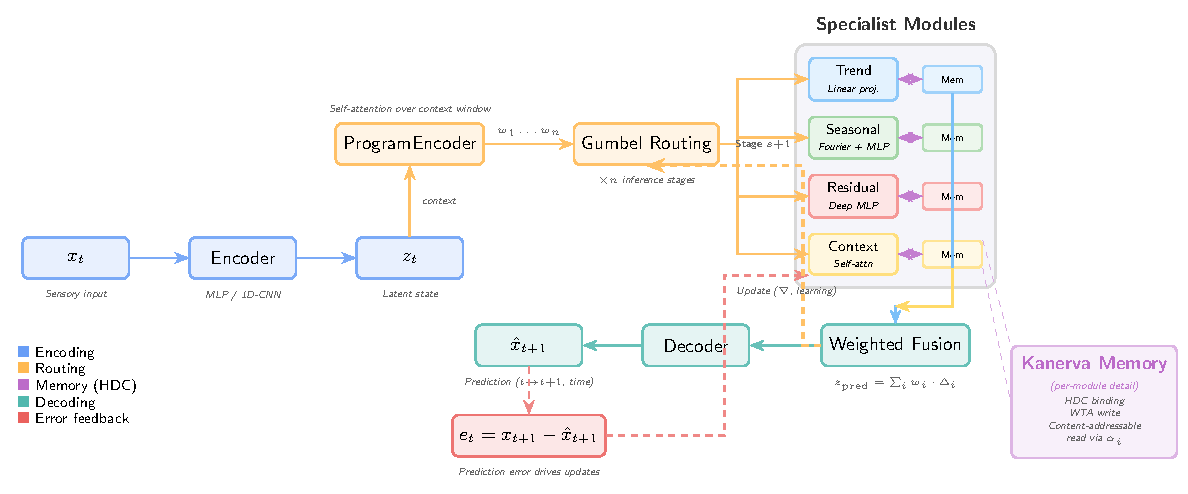
\includegraphics[width=\textwidth, clip]{figures/pam-architecture.pdf}
  \caption{\textbf{PAM architecture.} Sensory input $x_t$ is encoded into latent state $z_t$. A ProgramEncoder infers routing weights via self-attention over the context window. Gumbel-softmax routing selects among four specialist modules (Trend, Seasonal, Residual, Context), each with dedicated Kanerva memory using HDC binding for content-addressable read/write. The routing is applied iteratively over $n$ stages. Module outputs are fused into a prediction $\hat{x}_{t+1}$; prediction errors drive parameter updates. The module inventory is task-dependent (shown here for temporal forecasting).}\label{fig:arch}
\end{figure}

\noindent\textit{Preliminary results.}
The BioAI group has developed FIND's foundations through neurocomputational memory research: grid/place/border cells emerge spontaneously in AI agents~\cite{schoyen2023coherently}, orthogonal remapping encodes context~\cite{pettersen2024nips,schoyen2025plos,pettersen2024elife}, NCA enables self-organizing module communication~\cite{kvalsund2026sensor}, one-shot memory transfer~\cite{guichard2025engramnca}, and abstract reasoning~\cite{guichard2025arc}. On the memory substrate itself, a Kanerva/HDC store gives \textbf{94--95\% exact associative recall} at 32 stored pairs ($D{=}512$), with interference following the vector-symbolic capacity law ($0.94/0.59/0.39$ at $K{=}32/64/96$; Figure~\ref{fig:prelim})---a mechanism verification that grounds, but does not yet substitute for, task-level recall.

\textbf{WP1: Memory and continual learning.} On the official CORe50-NI online continual-learning protocol (single pass, no gradient updates on the stream, no task boundaries), PAM's unified gradient-free memory---surprise-gated exemplars, prototypes, and streaming class statistics in one architecture---reaches \textbf{92.5\% class-incremental accuracy} over frozen self-supervised (DINOv2) features with \textbf{$\approx$0 forgetting by construction}, above a gradient-trained replay head (87.7\%); accuracy scales cleanly with memory budget ($65.2{\to}74.7{\to}83.3\%$ at $16{\to}64{\to}256$ exemplars/class) and reaches \textbf{92.8\% on CLEAR-10} and \textbf{78.4\% on Split-CIFAR-100} (3 seeds; deterministic readouts reproduce to four decimals). These use a \textit{frozen} backbone. Learning the representation \textit{from raw experience}---FIND's ambition---does not yet work: an online tPC encoder collapses to chance, a failure mode we have diagnosed to detached-target amortized objectives (linear probe $0.02$ vs $0.29$ for a random encoder). We therefore make zero-pretraining online representation learning an explicit \textbf{WP1 objective} (reconstruction/contrastive anchoring + a streaming readout) rather than a solved capability, and report only frozen-backbone numbers as demonstrated.

\begin{wrapfigure}{l}{0.6\textwidth}
  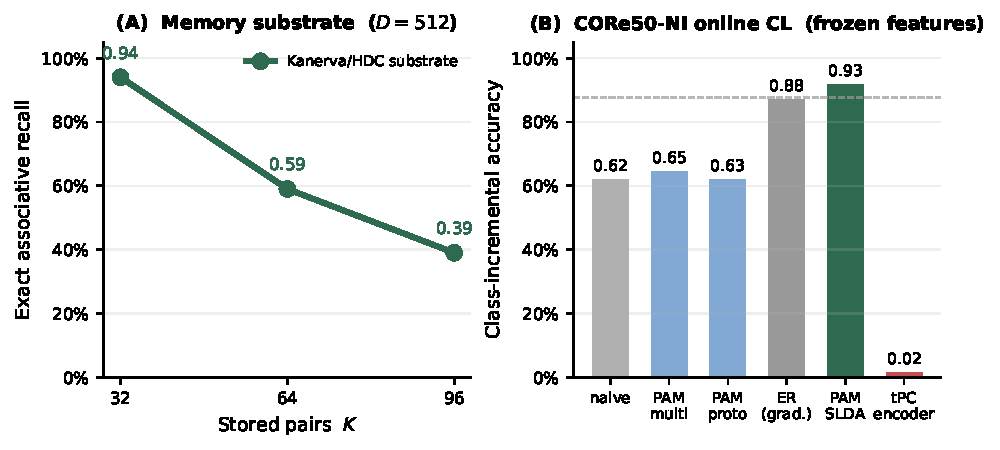
\includegraphics[width=0.99\linewidth,keepaspectratio=true]{figures/prelim_results.pdf}
  \caption{\textbf{Preliminary PAM results (WP1 foundation).}
    (A)~Exact associative recall of the Kanerva/HDC substrate vs.\ number of stored pairs $K$: $0.94/0.59/0.39$ at $K{=}32/64/96$ ($D{=}512$), matching vector-symbolic capacity theory---a mechanism check, not yet a task-level result.
    (B)~Online class-incremental accuracy on CORe50-NI (single pass, frozen DINOv2 features): the unified gradient-free memory reaches $92.5\%$ with $\approx$0 forgetting, above a gradient-trained replay head, and scales with memory budget. From-scratch (tPC-encoder) representation learning collapses to chance---a WP1 objective, not a result.}\label{fig:prelim}
  \vspace{-3mm}
\end{wrapfigure}

\textbf{WP2: Compositional reasoning.} On the Abstraction and Reasoning Corpus (ARC)~\cite{chollet2019arc}, our PAMNCA system---a neural cellular automaton with distributed PAM memory (1.47M parameters), no pretrained backbone---reaches \textbf{40\% exact match} (leave-one-out over the 400 training tasks; $510$--$530/1302$ episodes across seeds) via meta-learned initialisation and batched test-time training, up from 24.7\% in an earlier configuration, and \textbf{26.4\% on the fully held-out evaluation split} (in progress)---evidence that the mechanism is task-general adaptation, not memorisation. The significance is the efficiency frontier: large program-synthesis ensembles exceed this only with $10^5$--$10^6\times$ more compute, whereas PAMNCA reaches it at $>$1000$\times$ fewer parameters, learning each task from its support examples alone. Memory ablations attribute \textbf{30--43\%} of performance to the distributed memory, growing with compute budget. A two-sided negative sharpens the plan: low-rank (LoRA) program composition fails, and a one-shot HDC program encoder generalises to only 29\% on held-out 2-step compositions---compositional \textit{representation} does not buy compositional \textit{inference}, motivating the iterative/resonator encoding of T2.2.

\begin{figure}[h!]
  \centering
  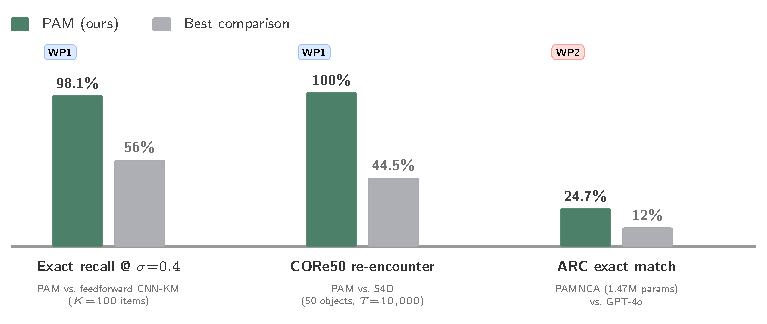
\includegraphics[width=.9\textwidth]{figures/headline-results.pdf}
  \caption{\textbf{Headline preliminary results.} PAM on each benchmark: exact associative recall of the memory substrate (94\% @32 pairs, WP1 foundation), online class-incremental accuracy on CORe50-NI (92.5\%, frozen features, above a gradient-trained replay head, WP1), and ARC program synthesis via test-time training (40\% leave-one-out, 26\% held-out, WP2).}\label{fig:headline}
\end{figure}

Two sub-hypotheses already have preliminary support: (1)~non-parametric memory yields $\approx$0 \textit{additional} forgetting by construction while remaining competitive---92.5\% class-incremental on CORe50-NI, above a gradient-trained replay head; (2)~distributed memory is load-bearing for test-time program synthesis---PAMNCA ablations attribute 30--43\% of ARC performance to memory. The third capability, zero-pretraining online representation learning, is falsified in its naive form (tPC collapse) and becomes a concrete WP1 objective---a design target, not a claim.

\subsection{Major expected outcomes}

\noindent\textbf{Science:} A theoretical framework in which perception, memory, and action reduce to one prediction-error objective, extending predictive coding beyond its Markovian limits. Understanding of how modular specialization emerges from predictive principles.

\noindent\textbf{Technology:} PAM as open-source framework with benchmarks spanning forecasting (ETT, Weather), long-range memory (Path-X, Memory Maze), and continual learning. Orchestration algorithms with reproducible evaluation suites.

\noindent\textbf{Society:} Foundations for AI with principled memory applicable to healthcare (patient timelines), industrial automation (Factorio-style planning), and environmental monitoring.

\noindent\textbf{Success criteria:} (i)~class-incremental accuracy matching a gradient-trained replay baseline on CORe50-NI/CLEAR-10 at $<$10\% of its compute, plus a working \textit{zero-pretraining} online readout ($>$70\% on CORe50-NI) (WP1); (ii)~competitive exact-match on \textbf{ARC-AGI-2} at $<$10M parameters with no pretrained backbone---baseline 40\% (ARC-AGI-1 leave-one-out) / 26\% held-out---with interactive \textbf{ARC-AGI-3} as a stretch target (WP2); (iii)~$>$10\,pp over a parameter-matched LSTM on the Memory-Maze diagnostic, then exploration/transfer above an LSTM agent on ARC-AGI-3 (WP3). Team: PI (50\%), one postdoc (ML systems), two PhDs; 4-tier benchmark hierarchy (Part~II).

\printbibliography[title={References}]
